\documentclass[UTF8]{ctexart}
\usepackage[a4paper,left=3cm,right=3cm,top=2cm]{geometry}
\usepackage{amsmath}
\usepackage{enumitem}
\usepackage{float}
\usepackage{threeparttable}
\usepackage{caption}
\usepackage{multirow}
\usepackage{graphicx}
\usepackage{listings}
\usepackage{xcolor}
\usepackage{amssymb}
\renewcommand{\figurename}{Figure}
\definecolor{dkgreen}{rgb}{0,0.6,0}
\definecolor{gray}{rgb}{0.5,0.5,0.5}
\definecolor{mauve}{rgb}{0.58,0,0.82}
\lstdefinelanguage{LC3}{
  morekeywords={ADD, AND, BR, BRn, BRnz, BRnzp, BRnp, BRz, BRzp, BRp, JMP, JSR, LD, LDI, LDR, LEA, NOT, ST, STI, STR},
  sensitive=false,
  morecomment=[l]{;},
  morestring=[b]",
  morekeywords=[2]{R0, R1, R2, R3, R4, R5, R6, R7}, % Define register keywords
}
\lstset{frame=tb,
  language=LC3,
  aboveskip=3mm,
  belowskip=3mm,
  showstringspaces=false,
  columns=flexible,
  basicstyle={\small\ttfamily},
  numbers=left,%设置行号位置none不显示行号
  numberstyle=\tiny\courier, %设置行号大小
  numberstyle=\tiny\color{gray},
  keywordstyle=\color{blue},
  keywordstyle=[2]\color{purple},
  commentstyle=\color{dkgreen},
  stringstyle=\color{mauve},
  breaklines=true,
  breakatwhitespace=true,
  escapeinside=`,%逃逸字符(1左面的键),用于显示中文例如在代码中`中文...`
  tabsize=4,
  extendedchars=false %解决代码跨页时,章节标题,页眉等汉字不显示的问题
}

\setlength\lineskiplimit{5.25bp}
\setlength\lineskip{5.25bp}

\title{Lab Report}
\author{崔士强 PB22151743}
\date{}

\bibliographystyle{plain}

\begin{document}

\maketitle
\section{Purpose}
The purpose of the program is to 

Anticipated outcomes:

\section{Principles}

\section{Procedure}
\subsection{Bugs encountered}

\subsection{Chanllenges}

\section{Results}
Results are shown below:
\begin{figure}[h]
        \centering
        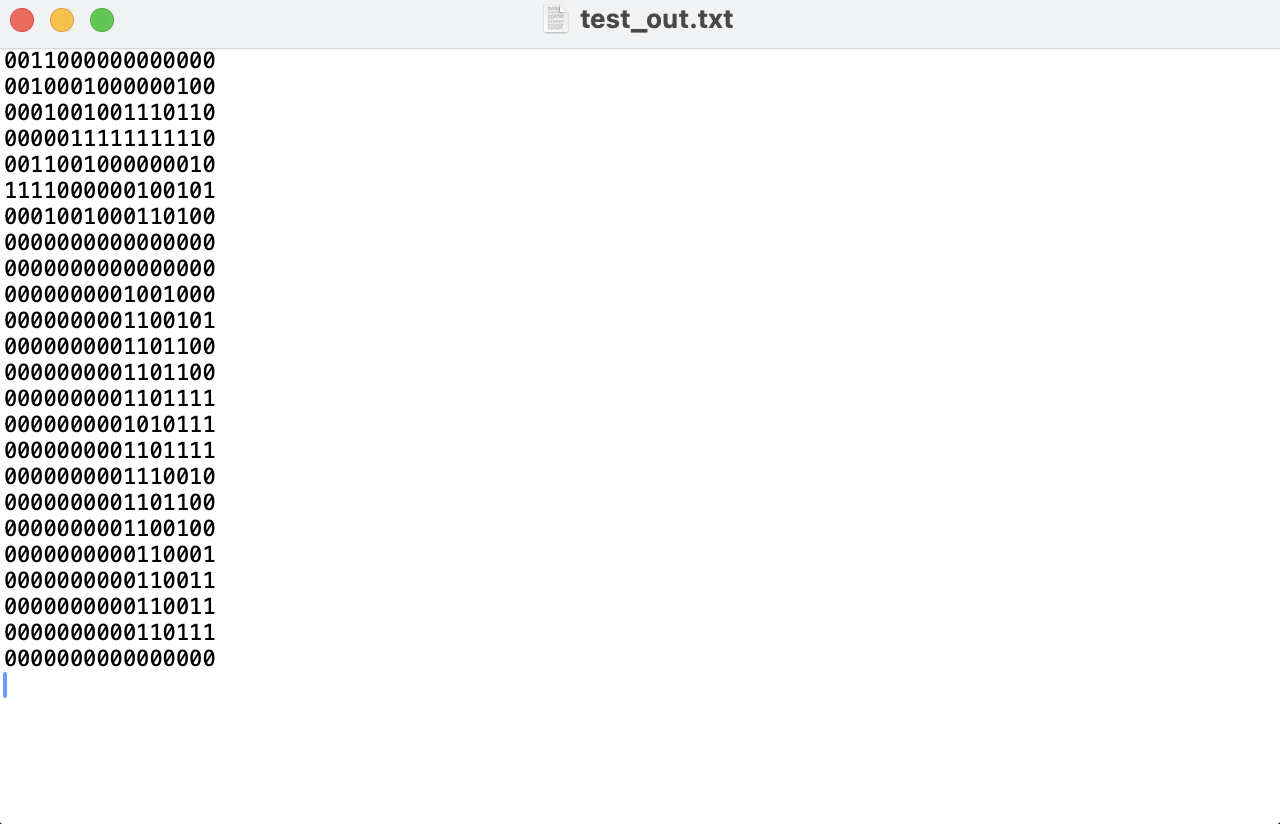
\includegraphics[scale=0.5]{result.png}
        \caption{Result}
\end{figure}

\section{Improvements}

\bibliography{math}

\end{document}
\iffalse
\begin{figure}[H]
    \centering
    \includegraphics[scale=0.5]{name.png}
    \caption{name}
\end{figure}
\fi
